%!TEX root = ../thesis.tex
%*******************************************************************************
%*********************************** Fourth Chapter *****************************
%*******************************************************************************

\chapter{Lattice Configurations and the Gluon Propagator}\label{chapter:GluonPropagator}
\ifpdf
    \graphicspath{{Chapter4/Figs/Raster/}{Chapter4/Figs/PDF/}{Chapter4/Figs/}}
\else
    \graphicspath{{Chapter4/Figs/Vector/}{Chapter4/Figs/}}
\fi

Now that we have developed the required background understanding of lattice QCD and the topological objects of interest to this research, we can explain how our calculations are performed. This chapter will first describe how we calculate the Landau gauge gluon propagator on the lattice. This is the primary quantity of interest for the first part of the original research, and as such we will explicitly detail its calculation.  We will then motivate our choice of momentum variables, before proceeding to a description of the renormalisation scheme we employ. Finally, we will present the lattice parameters and data cuts utilised in this work.

\section{Lattice Definition of the Gluon Propagator}
In a gauge field theory the position-space propagator, $D_{\mu\nu}(x,y)$, of the gauge boson is the two-point correlation function. In the case of perturbative QCD this can be interpreted as the probability amplitude of a gluon being created at the space-time point $x$, propagating to $y$, and then being annihilated. The propagator therefore serves as a useful measure of the behaviour of gluons as a function of distance; or, correspondingly, as a function of momentum in the momentum-space representation. In this section we detail how the non-perturbative momentum-space Landau gauge gluon propagator is calculated on the lattice. We begin with the definition of the coordinate-space propagator as a two-point correlator~\cite{Zwanziger:1991gz,Cucchieri:1999sz,Langfeld:2001cz}.
\begin{equation}
D^{ab}_{\mu\nu}(x) = \langle A^a_\mu(x) \, A^b_\nu(0)\rangle.
\label{eq:coordGluonProp}
\end{equation}
The propagator in momentum space is simply related by the discrete Fourier transform,
\begin{equation}
D^{ab}_{\mu\nu}(p) = \sum_x e^{-ip\cdot x} \langle A^a_\mu(x) \, A^b_\nu(0) \rangle. 
\end{equation}
Noting that the coordinate space propagator $D^{ab}_{\mu\nu}(x-y)$ only depends on the difference $x-y,$ such that
\begin{equation}
\langle A^a_\mu(x) \, A^b_\nu(0)\rangle = \langle A^a_\mu(x+y) \, A^b_\nu(y)\rangle\, ,
\end{equation}
we can make use of translational invariance to average over the four-dimensional volume to obtain the form for the momentum space propagator.
\begin{align}
D^{ab}_{\mu\nu}(p) &= \frac{1}{V}\sum_{x,y} e^{-ip\cdot x}\langle A^a_\mu(x+y) \, A^b_\nu(y) \rangle \nonumber \\
                &= \frac{1}{V}\sum_{x,y} \langle e^{-ip\cdot (x+y)} A^a_\mu(x+y) \, e^{+ip\cdot y}A^b_\nu(y) \rangle \nonumber \\
                &= \frac{1}{V}\langle A^a_\mu(p) \, A^b_\nu(-p) \rangle. \label{eq:gluPropxtop}
\end{align}

Hence we find that the momentum space gluon propagator on a finite lattice with four-dimensional volume $V$ is given by
%
\begin{equation}
D_{\mu\nu}^{ab}(p) \equiv \frac{1}{V}\left \langle A^a_\mu (p)\,A^b_\nu(-p)\right\rangle \, . \label{eq:gluonProp}
\end{equation}
%
In the continuum, the Landau-gauge momentum-space gluon propagator has the following form~\cite{Leinweber:1998im,Bonnet:2001uh}
%
\begin{equation}
D^{ab}_{\mu\nu}(p) = \left ( \delta_{\mu\nu} - \frac{p_\mu p_\nu}{p^2} \right )\,\delta^{ab}\,D(p^2) \, ,
\end{equation}
%
where $D(p^2)$ is the scalar gluon propagator.  Contracting Gell-Mann index $b$ with $a$ and
Lorentz index $\nu$ with $\mu$ one has
%
\begin{equation}
D^{aa}_{\mu\mu}(p) = (4-1)\,(n_c^2-1)\,D(p^2) \, ,
\end{equation}
%
such that the scalar function can be obtained from the gluon propagator via
%
\begin{equation}
D(p^2) = \frac{1}{3(n_c^2-1)}\,D^{aa}_{\mu\mu}(p) \, ,
\label{eq:scalarProp}
\end{equation}
%
where $n_c = 3$ is the number of colours.

As the lattice gauge links $U_\mu(x)$ naturally reside in the $3\times 3$ fundamental representation of $SU(3),$ we now wish to work in the matrix representation of $A_\mu(x)$, as introduced in Eq.~\eqref{eq:CovariantDerivative}. Using the orthogonality relation $\Tr(\lambda_a\lambda_b) = 2\delta_{ab}$ for the Gell-Mann matrices, it is straightforward to see that
%
\begin{equation}
2\Tr(A_\mu\,A_\mu) = A^a_\mu A^a_\mu\, ,
\end{equation}
%
which can be substituted into Eq.~\eqref{eq:scalarProp} to obtain the final expression for the lattice scalar gluon propagator,
%
\begin{equation}
D(p^2) = \frac{2}{3\,(n_c^2-1)\,V}\big\langle {\rm Tr}\, A_\mu(p)\,A_\mu(-p) \big\rangle \,. \label{eq:scalarProp2}
\end{equation}

To calculate Eq.~\eqref{eq:scalarProp2} on the lattice, we need to define $A_\mu(p)$. As defined in Eq.~\eqref{eq:GaugePotentialLat}, we make use of the midpoint definition of the coordinate-space gauge potential in terms of the lattice link variables such that
%
\begin{equation}
A_\mu\left(x+\frac{a}{2}\hat{\mu}\right) = \frac{i}{2ag}\left(U_\mu(x) - U_\mu^\dag(x)\right) - \frac{i}{6ag}\Tr\left(U_\mu(x) - U_\mu^\dag(x)\right)I + \mathcal{O}(a^2)\, .
\end{equation}
%
Once the link variables are fixed to Landau gauge following the procedure described in Sec.~\ref{sec:LandauGauge}, we can obtain the momentum-space gauge potential by performing a Fourier transform,
%
\begin{equation}
A_\mu(p) = \sum_x e^{-ip\cdot(x+\hat{\mu}/2)}\, A_\mu(x+\hat{\mu}/2)\, .
\end{equation}
%
We have now constructed a workable lattice definition to calculate the Landau gauge scalar gluon propagator within the lattice framework established in Chapter \ref{chapter:LatticeQCD}.

\section{Momentum Variables}\label{sec:MomentumVariables}
As discussed in Sec.~\ref{sec:Confinement}, it is understood that at high energies QCD is asymptotically free. With this understanding, we expect that at high momentum the Landau gauge gluon propagator will tend towards the Landau gauge photon propagator~\cite{ryder1996quantum}
%
\begin{equation}
D_\gamma(p^2) = \frac{1}{p^2}\, .
\end{equation}
%
However, lattice discretisation errors cause a deviation from this idealised behaviour that we would like to systematically account for. To do this, we follow the work of Refs.~\cite{Weisz:1982zw, Weisz:1983bn,Luscher:1985zq,Symanzik:1983dc,Symanzik:1983gh}. As we are considering the propagator at high momenta, it is sufficient to consider the behaviour of the photon propagator on the lattice. We therefore consider for this section only an Abelian theory. The commutator in the field strength tensor then vanishes, simplifying to
%
\begin{equation}
F_{\mu\nu} = \partial_\mu \,A_\nu - \partial_\nu\,A_\mu
\end{equation}
%
We consider this Abelian field to be on a lattice generated using the Wilson action (see Eq.~\eqref{eq:WilsonAction}). From Eq.~\eqref{eq:FieldStrengthPlaquette} we know that the Wilson action can be written as $\mathcal{S}_\text{W} = a^4\frac{1}{2}\sum_x F_{\mu\nu}F^{\mu\nu} + \mathcal{O}(a^4)$. As we are interested in the momentum-space propagator, we write the field strength tensor at the plaquette midpoint $\tilde{x}$ as
%
\begin{align}
F_{\mu\nu}(\tilde{x}) &= \frac{A_\nu\left(\tilde{x}+a\frac{\hat{\mu}}{2}\right) - A_\nu\left(\tilde{x}-a\frac{\hat{\mu}}{2} \right)}{a} - \frac{A_\mu\left(\tilde{x}+a\frac{\hat{\nu}}{2}\right) - A_\mu\left(\tilde{x}-a\frac{\hat{\nu}}{2} \right)}{a}\nonumber\\
&= \frac{1}{a} \sum_p e^{ip\cdot\tilde{x}} \left(\tilde{A}_\nu(p)\, e^{-iap\frac{\hat{\mu}}{2}} - \tilde{A}_\nu(p)\, e^{iap\frac{\hat{\mu}}{2}} - \tilde{A}_\mu(p)\, e^{-iap\frac{\hat{\nu}}{2}} + \tilde{A}_\mu(p)\, e^{iap\frac{\hat{\nu}}{2}}\right)\nonumber\\
&= -\frac{1}{a} \sum_p e^{ip\cdot\tilde{x}}\left(2i\sin\left(\frac{a p_\mu}{2}\right)\tilde{A}_\nu(p) - 2i\sin\left(\frac{a p_\nu}{2}\right)\tilde{A}_\mu(p)\right)\nonumber\\
&= - \sum_p e^{ip\cdot\tilde{x}}\tilde{f}_{\mu\nu}(p)\, ,
\end{align}
%
where
%
\begin{equation}
\tilde{f}_{\mu\nu}(p) = i\left(\hat{k}_\mu \tilde{A}_\nu(p) - \hat{k}_\nu \tilde{A}_\mu(p)\right)\, ,~\hat{k}_\mu = \frac{2}{a}\sin\left(\frac{ap_\mu}{2}\right)\, .
\end{equation}
%
The Wilson action can therefore be written as
%
\begin{align}
\mathcal{S}_\text{W} &= a^4\frac{1}{2}\sum_{\tilde{x}}\sum_{p,\,p^\prime}e^{i\tilde{x}(p+p^\prime)}\tilde{f}_{\mu\nu}(p) \, \tilde{f}^{\mu\nu}(p^\prime)\nonumber\\
&=a^4\frac{1}{2}\sum_{p,\,p^\prime} \delta(p+p^\prime)\tilde{f}_{\mu\nu}(p) \, \tilde{f}^{\mu\nu}(p^\prime) \nonumber\\
&= a^4\frac{1}{2}\sum_{p}\tilde{f}_{\mu\nu}(p) \, \tilde{f}^{\mu\nu}(-p) + \mathcal{O}(a^4)\, . \label{eq:WilsonMomentum}
\end{align}
%
We are now in a position to consider the propagator. Equivalent to the two-point correlator definition, the propagator is also the Green's function of the equations of motion, $M_{\mu\nu}$, satisfying
%
\begin{equation}
M_{\mu\nu}D^{\nu\lambda}(p) = \delta_\mu^\lambda\, .
\end{equation}
%
In the continuum, we can write the Abelian Lagrangian density in terms of momentum space variables as 
%
\begin{align}
\mathcal{L} &= \frac{1}{2}\tilde{F}_{\mu\nu}\,\tilde{F}^{\mu\nu}\nonumber\\
&= \frac{1}{2}(p_\mu\,\tilde{A}_\nu - p_\nu\,\tilde{A}_\mu)\,(p^\mu\,\tilde{A}^\nu - p^\nu\,\tilde{A}^\mu)\nonumber\\
&= (p^2\delta_{\mu\nu} - p_\mu\,p_\nu)\tilde{A}^\mu\,\tilde{A}^\nu\, ,
\end{align}
%
and hence
%
\begin{equation}
M_{\mu\nu} = (p^2\delta_{\mu\nu} - p_\mu\,p_\nu)\, .
\label{eq:ContEquationsOfMotion}
\end{equation}
%
However, it is understood that in the continuum the equations of motion are not invertible unless an additional gauge fixing term is added, with a gauge fixing parameter $\alpha$. Hence, the equations of motion for the photon field in momentum space are given by Eq.~\eqref{eq:ContEquationsOfMotion} with an additional gauge fixing term~\cite{ryder1996quantum}
%
\begin{equation}
M_{\mu\nu} = p^2\delta_{\mu\nu} - \left(1-\frac{1}{\alpha}\right)p_\mu p_\nu\, .
\end{equation}
%
By inspection, we see that Eq.~\eqref{eq:WilsonMomentum} for the lattice Wilson action will have the same equations of motion, with the substitution $p_\mu\rightarrow \hat{k}_\mu$. In turn, this gives the propagator
%
\begin{equation}
D_{\mu\nu}(p) = \frac{1}{\hat{k}^2}\left[\delta_{\mu\nu} + (\alpha-1)\frac{\hat{k}_\mu \hat{k}_\nu}{\hat{k}^2}\right]\, .
\end{equation}
Landau gauge corresponds to setting $\alpha=0$, so we find that
%
\begin{equation}
D_{\mu\mu}(p) = \frac{3}{\hat{k}^2}\, ,
\end{equation}
%
and therefore by comparison with Eq.~\eqref{eq:scalarProp} we see that
%
\begin{equation}
D(p^2) = \frac{1}{\hat{k}^2}\, .
\end{equation}
%
This suggests that for the Wilson action we should make the substitution $p_\mu\rightarrow \hat{k}_\mu = \frac{2}{a}\sin\left(a p_\mu/2\right)$ so that at tree-level we observe the expected behaviour of the gluon propagator.\\

A similar analysis can be performed for the L\"uscher-Weisz action used in this work, taking into account the contributions from the rectangle terms. The L\"uscher-Weisz action written in the same form as Eq.~\eqref{eq:WilsonMomentum} is~\cite{Weisz:1982zw}
%
\begin{equation}
\mathcal{L}_\text{LW} = a^4\frac{1}{2}\sum_p \left(1+\frac{1}{12}a^2\hat{k}^2\right) \tilde{f}_{\mu\nu}(p) \, \tilde{f}^{\mu\nu}(-p) + \mathcal{O}(a^6)\, .
\end{equation}
%
The equations of motion then become
%
\begin{equation}
M_{\mu\nu} = \left(\hat{k}^2 + \frac{1}{12}a^2\hat{k}^4\right)\delta_{\mu\nu} - \left(1-\frac{1}{\alpha}\right)\left(\sqrt{\hat{k}_\mu^2 + \frac{1}{12}a^2\hat{k}_\mu^4}\right)\left(\sqrt{\hat{k}_\nu^2 + \frac{1}{12}a^2\hat{k}_\nu^4}\right)\, .
\end{equation}
Therefore the propagator is
%
\begin{equation}
D_{\mu\nu}(p) = \frac{1}{q^2}\left[\delta_{\mu\nu} + (\alpha-1)\frac{q_\mu q_\nu}{q^2}\right]\, ,
\end{equation}
with
\begin{equation}
q_\mu = \sqrt{\hat{k}_\mu^2 + \frac{1}{12}a^2\hat{k}_\mu^4} = \frac{2}{a}\sqrt { \sin ^ { 2 } \left( \frac { p _ { \mu } a } { 2 } \right) + \frac { 1 } { 3 } \sin ^ { 4 } \left( \frac { p _ { \mu } a } { 2 } \right) }\, .
\end{equation}
%
In Landau gauge, this tells us that the tree-level form for the scalar propagator is
%
\begin{equation}
D(p^2) = \frac{a^2}{4 \sin ^ { 2 } \left( \frac { p _ { \mu } a } { 2 } \right) + \frac { 1 } { 3 } \sin ^ { 4 } \left( \frac { p _ { \mu } a } { 2 } \right)} = \frac{1}{q^2}\, .
\label{eq:LWCorrection}
\end{equation}\\
Given Eq.~\eqref{eq:LWCorrection}, in this work we make the variable substitution $p_\mu\rightarrow q_\mu$ to ensure that at high momentum the gluon propagator tends towards tree level as required.

\section{Renormalisation}\label{sec:Renormalisation}
Before plotting the propagator, it is essential to discuss the issue of renormalisation. On the lattice, we calculate the bare dimensionless propagator $D_B(q^2,\Lambda)$, as the lattice introduces an explicit regularisation parameter in the form of the momentum cutoff, $\Lambda = \pi/a$. This is related to the renormalised propagator $D_R(q^2,\mu)$ through the relation
%
\begin{equation}
D_B(q^2,\Lambda) = Z_3(\mu, \Lambda)\, D_R(q^2,\mu)\, ,
\label{eq:LatticeRenormalisation}
\end{equation}
%
where $\mu$ is the renormalisation scale. To obtain the renormalisation constant $Z_3(\mu, \Lambda)$, and therefore the renormalised propagator, it is necessary to enforce a renormalisation scheme. Here we employ the momentum space subtraction (MOM) scheme~\cite{Bowman:2004jm,Leinweber:1998uu,Bonnet:2001uh}, which requires that for some sufficiently large $\mu$
%
\begin{equation}
D_R(q^2,\mu)\big|_{q^2=\mu^2}=\frac{1}{\mu^2}\, .
\end{equation}
%
This sets the value of the renormalisation constant to be
%
\begin{equation}
Z_3(\mu,\Lambda) = \, \mu^2 \, D_B(\mu^2,\Lambda)\, ,
\end{equation}
such that
%
\begin{equation}
D_R(q^2,\mu) = \frac{D_B(q^2,\Lambda)}{\mu^2 \, D_B(\mu^2,\Lambda)}\, .
\end{equation}
%
This renormalised propagator is what we plot in e.g. Fig.~\ref{fig:UntouchedPropagator}, and will be denoted as simply $D(q^2)$ hereafter. The value of $\mu$ is arbitrary, however to make contact with perturbation theory it is necessary that it is sufficiently large such that it is outside the infrared region where the gluon propagator exhibits substantial deviation from perturbative behaviour. Furthermore, $\mu$ must be away from the momentum cutoff, as the renormalisation constant is only independent of the cutoff in the limit that the cutoff tends towards infinity~\cite{Bonnet:2001uh,Boucaud:2006pc}.  Once the renormalisation scheme has been imposed, it is then possible to connect the lattice results with those obtained from perturbation theory by connecting the renormalisation constant from the MOM scheme with those obtained from the renormalisation schemes used in perturbation theory.\\
 
The crux of this argument is that it is the renormalised propagator, not the bare propagator, that carries the physical meaning.  More generally, it is the shape of the propagator that carries meaning, and we are free to impose a scaling constant without changing the physical significance of the result. To facilitate comparisons between vortex-modified ensembles, we make use of the original $Z_3(\mu, \Lambda)$ obtained for the untouched propagator unless specified otherwise. Maintaining this consistency is sufficient to comment on the qualitative shape of the propagator, which is the most significant point of interest in this research.\\

\section{Lattice Parameters and Data Cuts} \label{sec:LatticeParameters}
We calculate the gluon propagator on 100 configurations of a $20^3\times 40$ $SU(3)$ lattice with spacing $a=0.125\,\si{fm}$, as used in Refs.~\cite{Trewartha:2015nna,OMalley:2011aa}. The momentum variables chosen for both the Wilson and L\"uscher-Weisz action have been numerically verified to provide better tree level agreement in Refs.~\cite{Marenzoni:1994ap, Bonnet:2001uh}, and we present a comparison of the L\"uscher-Weisz and uncorrected variables in Fig.~\ref{fig:MomentumComparison}. To visualise this improvement, we plot $k^2\,D(k^2)$ (where $k_\mu=p_\mu,\,q_\mu$ is the momentum variable for the given case under consideration) such that the tree-level propagator appears as $k^2\,D(k^2)=1$, shown as the black dashed line. This choice of plotting $k^2\,D(k^2)$ against $ka$ has the benefit of aiding both the visualisation of the tree-level behaviour, and the onset of the non-perturbative infrared properties of the propagator. Via the method described in the previous section, we have renormalised the L\"uscher-Weisz corrected propagator such that $q^2\,D(q^2) = 1$ at $qa=6.0$, and applied this same renormalisation constant to the uncorrected propagator. While this choice of renormalisation point is near the cutoff, it provides a renormalised propagator that approaches tree-level from above. In subsequent sections we will select renormalisation points further away from the cutoff.\\

We can clearly see that at high momenta the corrected gluon propagator tends towards the expected tree-level behaviour, whereas the uncorrected propagator fans out considerably. This fanning is the result of asymmetry between the spatial and temporal components of the propagator, which is accounted for in the tree-level correction~\cite{Marenzoni:1994ap}. The results presented in Fig.~\ref{fig:MomentumComparison} clearly motivate the need for tree-level correction when calculating the gluon propagator on the lattice.\\ 
%
\begin{figure}[H]
\centering
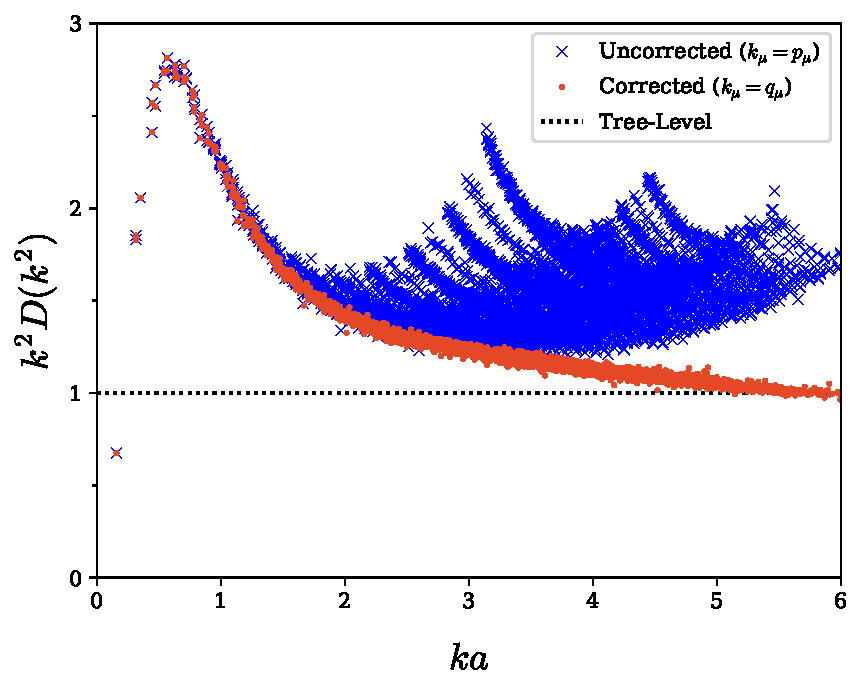
\includegraphics[width=\linewidth]{./ScalarGluComp_q2_MomentumComparison.pdf}
\caption[The renormalised scalar gluon propagator is plotted with no tree-level momentum correction and the L\"uscher-Weisz correction.]{\label{fig:MomentumComparison} The scalar gluon propagator is plotted with no tree-level momentum correction (blue crosses) and the L\"uscher-Weisz correction (red dots) presented in Eq.~\eqref{eq:LWCorrection}. It is clear that the corrected momentum has improved tree-level behaviour, free from the fanning effect present in the uncorrected case.}
\end{figure}
%

When considering the gluon propagator we shall maintain the plotting convention introduced in Fig.~\ref{fig:MomentumComparison} of considering $q^2D(q^2)$ against $qa$ for the remainder of this work. To improve the momentum-corrected propagator presented in  Fig.~\ref{fig:MomentumComparison} we follow the procedure of Ref.~\cite{Bonnet:2001uh,Leinweber:1998im} and perform a momentum half-cut. The momentum half-cut corresponds to only considering lattice momenta in the range
%
\begin{equation}
p_\mu = \frac{2\pi n_\mu}{a N_\mu},~n_\mu\in \left(-\frac{N_\mu}{4},\,\frac{N_\mu}{4}\right]\, .
\end{equation}
%
This cut limits the positive range of the kinematically corrected $q_\mu$ to
%
\begin{equation}
q_\mu \in \left[0,\, \frac{2\sqrt{21}}{3a}\right]\approx\left[0,\frac{3.06}{a} \right]\, .
\end{equation}
%
Furthermore, a cylinder cut of radius $pa=2$ lattice units is performed, such that we only consider points within two lattice units of the diagonal. This cut is implemented by considering points satisfying
%
\begin{equation}
|pa|^2\, \sin(\theta_c) \leq 2\, ,
\end{equation}
%
where
%
\begin{equation}
\theta_c = \cos^{-1}\left(\frac{pa \cdot \hat{n}}{|pa|}\right)\, ,
\end{equation}
%
and $\hat{n} = \frac{1}{2}(1,\,1,\,1,\,1)$ is the unit vector along the diagonal. This is performed so that all directions are equally sampled, whilst omitting points where one direction dominates the signal. This reduces the impact of lattice cutoff artefacts. Finally, we can take advantage of the rotational symmetry of the scalar propagator to perform $Z(3)$ averaging over the Cartesian coordinates. This means that we average over all points with the same Cartesian radius; for example, we would average across the points $(n_x,n_y,n_z)=(2,1,1),\,(1,2,1)$ and $(1,1,2)$. These choices of cuts assist in producing a cleaner signal that accurately represents the behaviour of the continuum propagator. With the momentum half-cut, we now renormalise at $qa=3.0$. This choice of renormalisation point is both sufficiently large and away from the lattice momentum cutoff, as well as falling within the momentum half-cut range of $qa\in [0,\,3.06]$. This choice of renormalisation point will be used for the remainder of this work.\\

With these cuts implemented, the gluon propagator on the original untouched configurations appears as Fig.~\ref{fig:UntouchedPropagator}. We observe the expected tree-level behaviour at high momenta, with an infrared enhancement indicative of amplified low-momentum propagation. It should be noted that the difference in peak height observed between Fig.~\ref{fig:MomentumComparison} and Fig.~\ref{fig:UntouchedPropagator} is due to the different renormalisation constant. Due to the cuts we have made, we observe a much cleaner signal, particularly in the region $qa\geq 1.5$, in agreement with the results of Ref.~\cite{Bonnet:2001uh}. For the remainder of this work we will employ these data cuts and this choice of momentum variables when plotting the gluon propagator to ensure an accurate and clear signal.
%
\begin{figure}
\centering
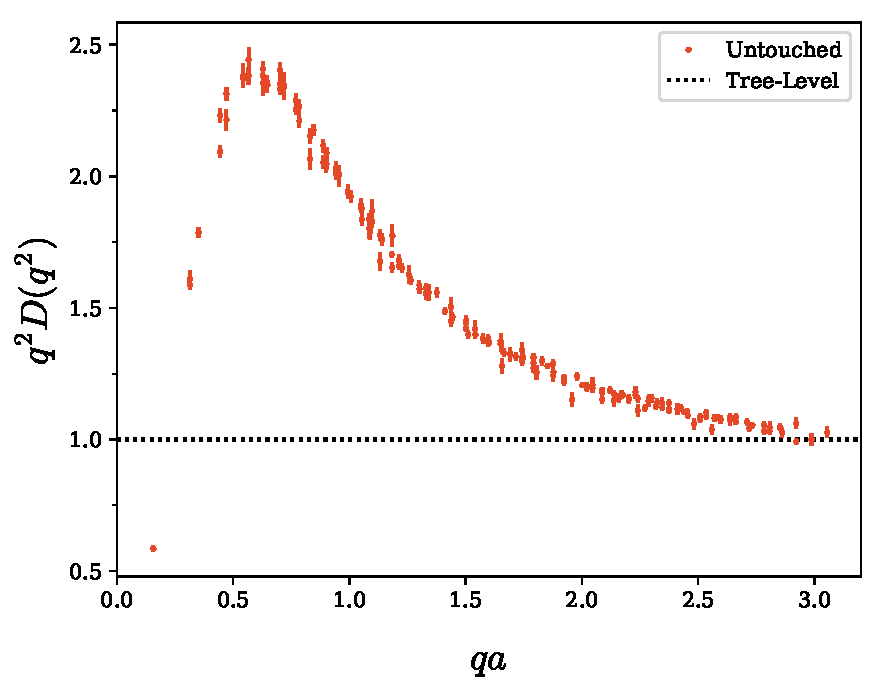
\includegraphics[width=\linewidth]{./ScalarGluComp_q2_NoCoolU.pdf}
\caption[The untouched gluon propagator with all data cuts and correct momentum variables utilised.]{\label{fig:UntouchedPropagator} The untouched gluon propagator with all data cuts and correct momentum variables utilised. We observe a substantially cleaner signal when compared to the untouched propagator shown in Fig.~\ref{fig:MomentumComparison}.}
\end{figure}


